\title{Gravitational Wave Detection in Gaussian Noise using Deep Learning}
\author{
        Pascal Müller [pamuelle@student.ethz.ch] \\[4cm]
        A bachelor thesis supervised by\\[2cm]
        Prof. Lavinia Heisenberg
}

\date{\today}

\documentclass[12pt]{article}
\usepackage[utf8]{inputenc}
\usepackage{graphicx}
\usepackage{pdfpages}
\usepackage{hyperref}
\usepackage[parfill]{parskip}
\usepackage{amsmath}
\usepackage{hyperref}
\usepackage{soul}
\usepackage{multirow}

\usepackage{tikz}
\usetikzlibrary{shapes,arrows}

\usepackage{biblatex} %Imports biblatex package
\addbibresource{src/references.bib} %Import the bibliography file

\definecolor{LightGray}{gray}{0.9}

\newcommand{\hlc}[2][LightGray]{{%
    \colorlet{foo}{#1}%
    \sethlcolor{foo}\hl{#2}}%
}

\begin{document}
\maketitle

%!TEX root = ../thesis.tex

% TODO:
% 1. Improve quality.
% 2. Make sure we have a reference for everything. (e.g. add einstein paper)
% 3. Finish the "organized" part at the end.
% 4. Improve quality of Figure 1.
% 5. Maybe add that this is the basic for a project where new physics should
%    be found like e.g. NS eq. of state blabla.

\section{Introduction}
% Introduction to the general topic of GW
In 1916, Einstein predicted the existence of gravitational waves (GW). Nearly
100 years later, on September 14, 2015, the first detection of a gravitational
wave\cite{PhysRevLett.116.061102}, emitted by two merging black holes, confirmed
his prediction. This detection marked the beginning of the GW astronomy era.
Until then, it was also the last missing extrasolar messenger needed for 
full-scale multi-messenger physics.
\cite{Branchesi_2016} 

% Multi-Messenger physics: Importance of latency
Because multi-messenger physics utilizes different messengers to observe the 
same transient, it is of paramount interest to minimize the latency between 
the detector measuring the GW and its reported detection. This allows for
fast follow-up observations of the other messengers.

% Descibe the current situation: We have several detectors. The measurement is
% noisy.
When analyzing the \textit{strain} $h(t)$ measured by the detector, the
fundamental assumption is that it is made up by the GW \textit{signal} $s(t)$
and \textit{noise} $n(t)$ whereas

\begin{equation}
  h(t) = n(t) + s(t)
\end{equation}

Analyzing $h(t)$ about the possible occurence of $s(t)$ is currently done by
using an approach called matched filtering. Matched filtering works by 
convoluting precalculated models of expected signals, so called templates, with
the measured data generating a signal-to-noise (SNR) time series. Because the
parameters of the expected signals are not known in advance, the template bank
spans a large astronomical parameter space.
Using a SNR threshold, we can extract \textit{triggers} marking possible GW 
signals. Clustering together close triggers leads to a \textit{candidate event}.

Convoluting the measured data with the whole template bank is computationally
expensive, which in turn leads to a high latency between data aggregation and
the reported detection. This motivates the search for methods which are less
computationally expensive and thus provide a low-latency detection algorithm.

\begin{figure}[ht]
  \includegraphics[width=0.95\textwidth]{img/1_introduction/data_processing.png}
  \caption{A simplified schematic summarizing the main steps in LIGO-Virgo data
           processing, from the output of the data to the results reported in a
           catalog of transient events.}
  \label{fig:1_data_processing}
  \centering
\end{figure}

In \autoref{fig:1_data_processing}, taken from \cite{2020CQGra..37e5002A},
we can see a simplified schematic summarizing the main steps in LIGO-Virgo data
processing. The detectors are highly sensitive which makes them prone to
different noise sources. One observed phenomenon are so called glitches which
can mimic true transient astrophysical signals \cite{2020CQGra..37e5002A}.
After a quality control, the data is being searched for GW signals and in case
a signal is found, called an candidate event, the parameters are being estimated.

Each candidate event gets a statistical significance assigned, which is given by the 
false-alarm rate (FAR) of the search. The FAR is basically telling us how many false positives
occured over the duration of the analyzed data. To count the amount of
false positives, we use the ranking statistic, given by the maximal SNR
of the considered candidate event, as the threshold. Current low-latency searches
do not distribute any event candidates with a FAR greated than 1 per month.
\cite{PhysRevD.98.024050}

In their pioneering works, \citeauthor{PhysRevD.97.044039} \cite{PhysRevD.97.044039}
and \citeauthor{PhysRevLett.120.141103} \cite{PhysRevLett.120.141103} showed
that convolutional neural networks (CNN) can be used to distinguish between
pure noise and noise containing a GW signal. Both works use a classical binary
classification framework where they utilize the \textit{false alarm probability}
(FAP) to compare their results to matched filtering. Applying matched filtering
on fixed sized samples to compute the FAP and using it to compare the two
approaches is problematic because the matched filtering approach used in the 
LIGO-Virgo data processing pipeline acts on a time series of arbitrary length
resp. on a continous data stream. \cite{PhysRevD.100.063015}

In this thesis, we will explore a similar deep learning (DL) approach to search,
for simulated GW signals in simulated white gaussian noise. While training a 
neural network (NN) is also rather computationally expensive, the evaulation of
a trained NN can be done in a fraction of a second. Furthermore future 
detections can easily be incorporated leading to an improved neural network.

This thesis is organized as follows. In Section 2 we first establish the data
used for our DL approach, so we know what we actually work with. In section 3 
we will describe the actual DL approach. In section 4, we present the results.
In section 5 we discuss possibilities for future work.

TODO: 
\begin{itemize}
  \item Figure 1: Better quality needed
  \item Text: Quality control
  \item Do I need to add a paragraph about the "openness" of the thesis?
  \item Do I need to comment about the generalilty of the code?
  \item "This thessi is the basis of a project"?
\end{itemize}




%!TEX root = ../thesis.tex

\section{Data Generation}
% Give quick intro into what kind of data is needed for a DL approach.
In deep learning, one basically tries to fit a mathematical model, the neural
network, to a data set consisting of measurements. This process is called
\textit{learning}.
Those measurements might be data from a physical experiment, time series from
the stock market, health information collected for mice or virtually any
other source of data.

In most cases, the data is split into three sets. The first subset is used to
train the neural network and is called \textit{training set}. The second subset 
is used to validate the learning progress and is called \textit{validation set}.
This process of learning and validating is repeated until we think the trained
NN can make good predictions. In a last step we use the trained NN to make an
unbiased prediction on the third subset, called \textit{test set}.

In the case of GW we only have a very limited data set of measurements. We can't
make an experiment to easily generate more measurements, we can only try to 
detect the ones which occure naturally. This rises the problem of needing to 
know how a gravitational wave looks like to be able to measure it. We solve this
by simulating GW waveforms and injecting it into Gaussian noise.

\subsection{Training and Validation Set}
% Parameters for signal
To generate the training and validation set, we first generate $100'000$ GW signal
waveforms sampled at 2048 Hz. The two masses $m_1$ and $m_2$ are drawn uniformly
between $10 \textup{M}_\odot$
and $50 \textup{M}_\odot$ whereas $m_1 < m_2$. The \textit{coalescence phase},
\textit{inclination} and \textit{polarization angle} are drawn uniformly between
$0$ and $2 \pi$. Furthermore we use
pyCBC's \hlc{sky\_location.UniformSky()} to compute the \textit{declination} and
\textit{right ascention}. We also use a \textit{low frequency cutoff} of 18 Hz.
We use the \hlc{SEOBNRv4\_opt} approximant to generate the waveforms. Those
choices are motivated by \cite{PhysRevD.105.043002} and \cite{MLGWSC1}. 
Note that here, the sky 
location as well as the inclination and polarization are set from the start.

The NN which will be used in this thesis \cite{PhysRevD.105.043002} assumes
the training and validation set to cointain 1 second long samples yet the 
generated waveforms will end up having 
a duration of several seconds. We solve this problem by choosing a 1.25 second
window around the merger. This leads to the merger being always placed in
the middle of the window. Since a NN is likely to learn such positional
information, we vary the placement of the window randomly by 0.2
seconds. This way, the mergers placement won't be fixed, adding stability to our
NN. \autoref{fig:2_cutting_windows} shows three such choices for a
window containing the merger whereas green is the maxiaml variation towards the
left, red is without variation and yellow is the maximal variation towards the
right. Limiting the variation by 0.2 seconds is an arbritary choice.

\begin{figure}[t]
  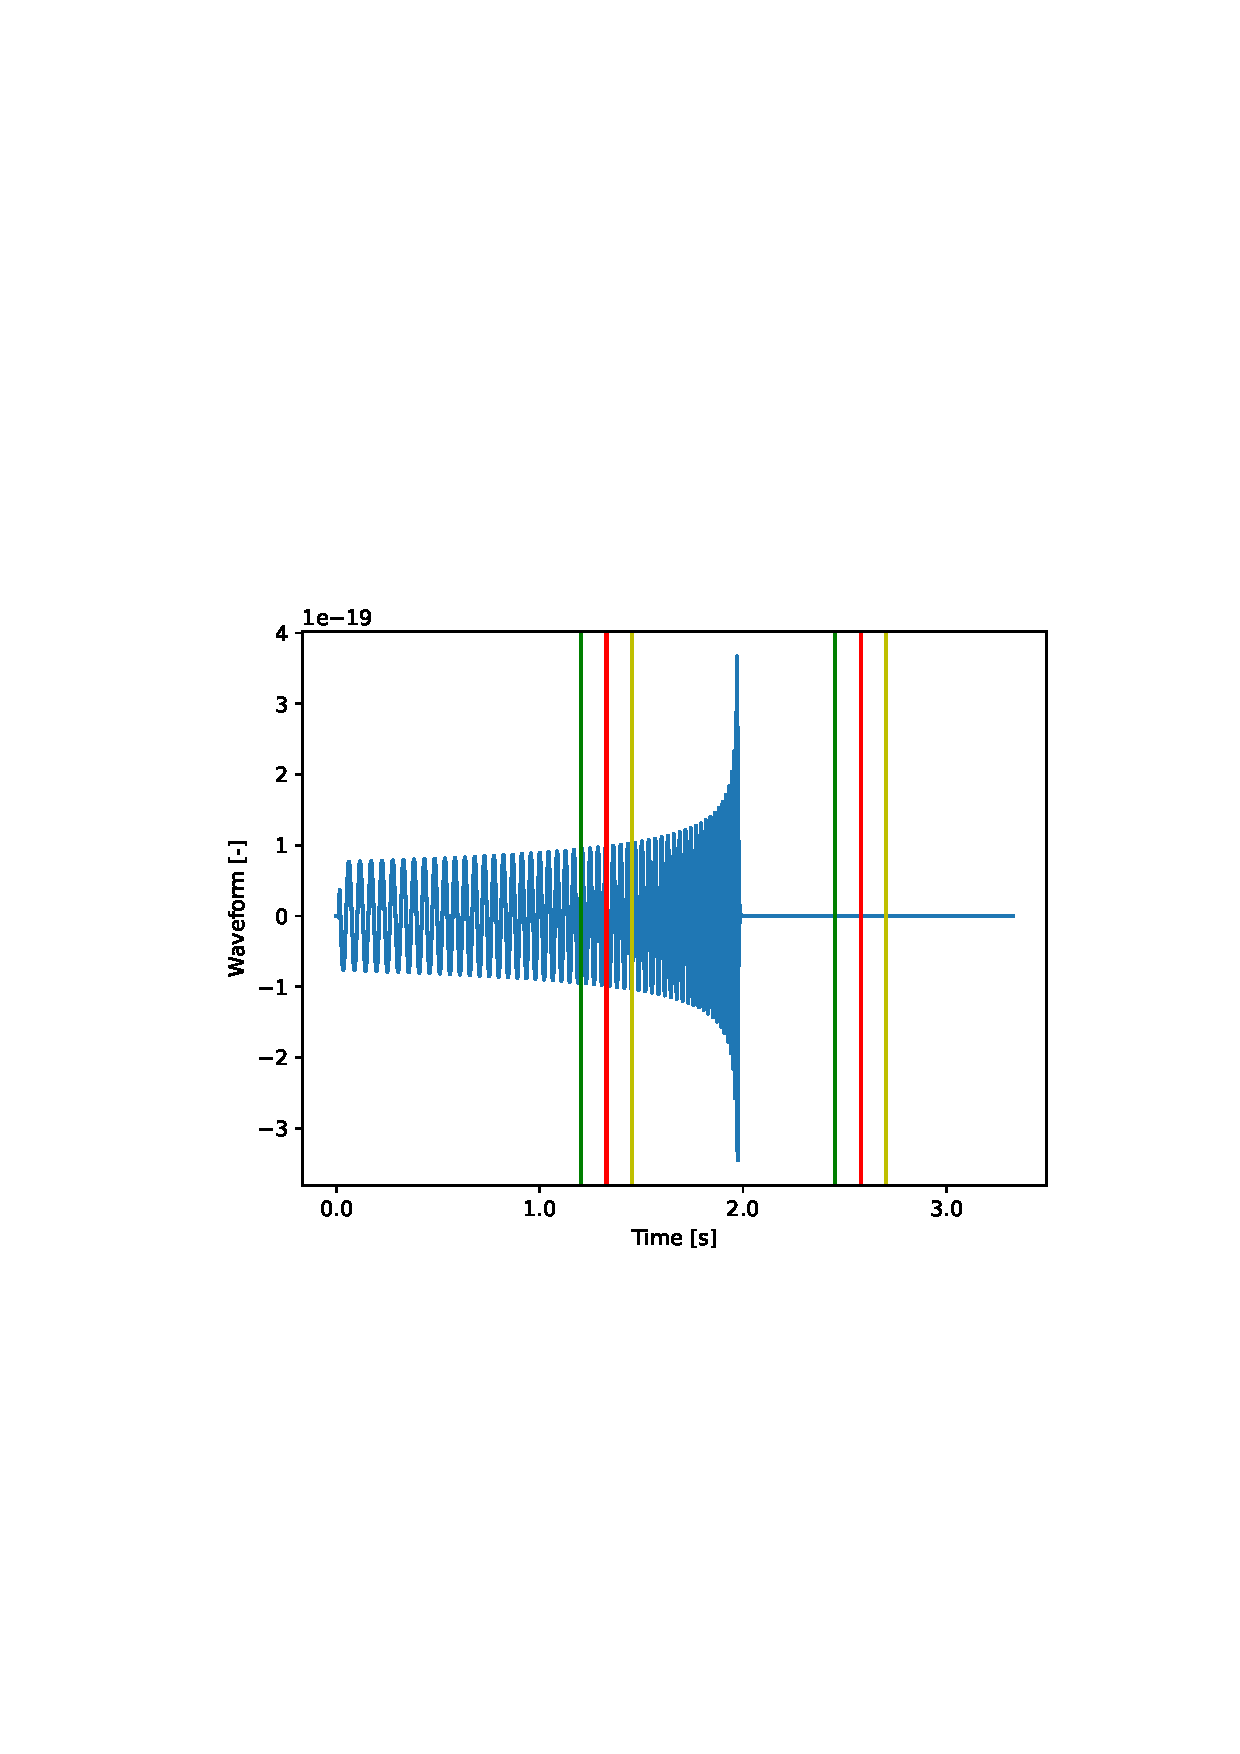
\includegraphics[width=\textwidth]{img/2_data_generation/chapter2_cutting_window.png}
  \caption{Cutting windows varied by \textcolor{green!40!black}{-0.2s},
    \textcolor{red}{0.0s} and \textcolor{yellow!60!black}{+0.2s}}
  \label{fig:2_cutting_windows}
  \centering
\end{figure}

% Parameters for noise
Next we generate $200'000$ pure Gaussian noise samples sampled at 2048 Hz with
a duration of 1.25 seconds.
The noise is generated using pyCBC's implementation of
\hlc{aLIGOZeroDetHighPower} PSD with a low frequency cutoff of $18$ Hz
\cite{PhysRevD.105.043002} \cite{MLGWSC1}.

% Generating samples
At last we need to generate the actual samples used to train and validate the NN
. This is done by injection all $100'000$ signal waveforms into $100'000$ of the
$200'000$ noise samples. We end up with $100'000$ pure Gaussian noise samples
and $100'000$ samples of signals injected into Gaussian noise.

From \cite{PhysRevD.105.043002} we see that the best training is done on samples
with SNR
of 8. This is because DL algorithms can generalize low SNR signals to high SNR
ones while the converse is not true. \cite{PhysRevD.105.043002} 
Because of this, we rescale
the signals to have an SNR of 8 before injecting them into the Gaussian noise.

In a last step, all $200'000$ samples are whitened, leading to corrupted edges.
Removing the corrupted edges reduces the duration of each sample from
1.25 second to 1 second. This corruption of the edges happens because the
algorithm implementing whitening
assumes periodicity of the data while the data isn't periodic. This assumption
stems from the fact that analtically, whitening assumes an infinite time series.
\footnote{Discussed with Ondřej Zelenka on 10.12.2021 in a private Slack
  conversation.} 

We end up with $200'000$ samples of 1 second whereas half of it contains a signal
and the other half doesn't. We say they have the labels \textit{pure noise} and 
\textit{noise+signal}. Those $200'000$ samples will then be split into
training and validation set using a 80/20 split. Before the split, the samples
are shuffled uniformly leading to a similar ratio between
pure noise and noise+signal samples in both sets. There is no mechanism in place
to enforce an equal ratio.

\subsubsection{Implementation}
Generating the above described data is implemented in the file \\
\hlc{generate\_training\_data.py} found in the \hlc{scripts} folder. It utilizes
the classes \hlc{SignalSpace}, \hlc{SignalGenerator}, \hlc{NoiseSpace},
\hlc{NoiseGenerator}, \hlc{SampleSpace} and \hlc{SampleGenerator}. We can divide
all those classes into two categories: \hlc{Spaces} and \hlc{Generators}. The
\hlc{Spaces} provide the parameters used to generate noise, signals or samples
and the \hlc{Generators} takes one set of parameters to generate the noise,
signal or sample using its \hlc{generate(params)} method.

The data generation is a computationally expensive task. If implemented
sequentially\footnote{Sequentially means one task is executed after the other,
basically running it on one core.} it can take
up to a day or even longer, depending on the approximant used and the
amount of data generated. To drastically reduce the time needed for data
generation, I parallelized\footnote{Parallelization is the task of implementing
an algorithm in a way such that it can run on several cores simultaneously.
Reducing its execution time.} it using a \textit{master-slave} approach
implemented using MPI\footnote{resp. the Python wrapper mpi4py}. In
this approach one core, the master, distributes a batch of work and the slaves
execute this batch of work. Once a slave is done it asks the master for more
work.

This approach was chosen because the computational work differs from
sample to sample which means that if we were to distribute all the work in the
beginning, we wouldn't utilize the full power of all cores. Furthermore this
approach also made it easy to ensure that
all work is generated from the same \hlc{Space} (i.e. distribution) which is
important because we use several random number generators. This choice
also gives a lot of flexibilty, which is important when working with DL since
it allows you to easier iterate over ideas.

The data generation was run on ETH's Euler cluster which acts as a distributed
system and is the reason we chose MPI instead of e.g. openMP to parallelize the
data generation.

\subsection{Test Set}
The test set consists of 1 month of data. Note that this is different to the
training and validation set since those used samples of a duration of 1 second
while here we basically have one sample with a duration of 1 month. This is
needed to address the issues describes in \cite{PhysRevD.100.063015}.

The test set is being generated by utilizing the \hlc{generate\_data.py} script
from \cite{MLGWSC1}. Note that \cite{MLGWSC1} provides the possibility of
generating test data on 4 complexity level. The first one being Guassian noise
and simulated signals while the last one is basically real LIGO-Virgo data.

The reason it was used is because it gives the possibility to easily test the
trained NN on more complex test data. Note that in this thesis, only the simplest
test set was used.

This script will generate two datasets. One fore the so called
\textit{foreground data} and another for the so called \textit{background data}.
The difference is that the background data only contains the pure noise
while the foreground has signals injected into it as described in the
\textit{injections} file. Having both files allows us to conpate false positives
with true positives which in turn is needed to compute metrics.

Note that a LIGO observation run is split into time segments which indicate
the time intervals in which the measured data was of sufficient quality. While
the injections file contains injections for the whole duration of an
obervation run i.e. ignores the segments, the \hlc{generate\_data.py} script
only chooses injections which are at a time contained in one of the segments. In
the generated HDF file, each such segment is stored in its own dataset.

Since our training data consists of whitened samples, we also have to whiten the
test data. This is done by whitening each segment at once, again resulting in a
data loss of $0.25$s for each segment. In total, we lose $32.5$ seconds after
whitening the whole month of data. Whitening here is done by the \hlc{whiten.py}
script provided in \cite{MLGWSC1}. This script again utilizes the \hlc{whiten}
function of pyCBC but also allows you to provide the noise PSD explicitly. In
case it isn't provided explicitly, it tries to estimate it from the given strain
. Having these features is especially important when working with the more
complex data sets.


%!TEX root = ../thesis.tex

\section{Deep Learning Approach}
% Introduction: High-level overview about general idea behind DL.
% Main Workflow: Describe the main workflow (train + eval in each epoch)
% Training: Describe training
% Evaluation: Describe evaulation (incl. accuracy and efficiency)

% Quick introduction to deep learning
Deep learning is a machine learning approach which consists of processing
units, so called neurons, which are arranged in an array. Such an array makes up
a layer. One to several such layers make up a neural network (NN). Each neuron
acts like a filter extracting higher-level features from the raw input. On a 
basic level, a neural network is trained by repeatedly applying the training
data and comparing its results with the known labels.

% Extend on the introduction
For the DL approach one needs a training set and a test set. The training set
is split whereas 80\% is used for the actual trianing of the NN and 20\% is used
to evaluate the trained NN in each epoch. 

% Provide pseudo code for main workflow
As we can see in pseudocode X, we havet his workflow. yada yada yada

% Provide pseudo code for train()

% Provide pseudo code for validation()



In this thesis the neural network from \cite{schaefer2021training} is used.
TODO: FAR like used in gabbart et al is "wrong", so use ml strategies approach.




%!TEX root = ../thesis.tex

\section{Results}
In \autoref{fig:4_losses} we can see the evolution of training and validation
loss during a 200 epochs run. In this run, the NN as described in chapter 3 and
the training data as described in chapter 2 was used. The NN converges fast
until about epoch 60. After epoch 60 training and validation loss start to
slowly diverge, indicating that the NN started to overfit on the training data.
Apparently it even converges a little bit faster than the corresponding 
experiment in \cite{PhysRevD.105.043002}.
\footnote{According to Ondřej Zelenka in a private discssion on Slack on
  24.01.22} I accord this to the difference in training set. The state of the
NN at epoch 59 was chosen as the \hlc{best\_weights.pt}.

\begin{figure}[ht]
  \includegraphics[width=\textwidth]{img/4_results/losses.png}
  \caption{Training and validation loss over 200 epochs.}
  \label{fig:4_losses}
  \centering
\end{figure}

In \autoref{fig:4_eff} we can see how the efficiency evolved over the 200 epochs.
Again we have a fast improvement of the efficiency and after about epoch 40 it
converged to about 0.9, which is similar to what the authors of
\cite{PhysRevD.105.043002} observed.

\begin{figure}[ht]
  \includegraphics[width=\textwidth]{img/4_results/efficiencies.png}
  \caption{eff.}
  \label{fig:4_eff}
  \centering
\end{figure}

The low loss as well as the high efficiency are good indicators for a good
performance of our NN. To evaluate how good the NN actually is, two numerical
experiments were made. The first one was applying the network to a small test
set with short duration. The second one was applying the neural network to test
data of 1 month and computing a sensitivity plot.

\subsection{Experiment 1: Short Test Data}
In this experiment, a short strain of noise was generated and injected with 5
signals at different SNR. The whole strain was whitened and analyzed by the
neural network.

In \autoref{fig:4_apply_single} we can see a plot consisting of three windows.
The top window displays pure noise in blue with the 5 signals overlayed. Note
that it does in the top window, the signals are not yet injected into the noise.
In the middle window, we can see the whitened noise+signal strain. In the bottom
window, the p-score of the network is plotted.

As we can see, the network detects all signals and assigns a pscore of 1 for all
of them but it sometimes also assigns a high pscore value to noise. Noteworthy
is also the difference between the thickness of the bars in the bottom window.
The bars indicating signals are thicker because we use a sliding window to feed
the data to our NN, leading to several windows containing the same merger.

The result to this experiment made me confident, that the NN does indeed
recognize GW signals injected in whitened Gaussian noise.

\begin{figure}[ht]
  \includegraphics[width=\textwidth]{img/4_results/apply_single.png}
  \caption{apply single.}
  \label{fig:4_apply_single}
  \centering
\end{figure}

\subsection{Experiment 2: 1 Month of Test Data}
In this experiment, we analyze a month of test data, compute the FAR as well as
the sensitive distance and plot it. Computing the FAR as well as the
sensitivity distance is done with code prodived by \cite{MLGWSC1}.

\begin{figure}[ht]
  \includegraphics[width=\textwidth]{img/4_results/sensitivity_plot.png}
  \caption{The NN applied to short test data.}
  \label{fig:4_sensitivity_plot}
  \centering
\end{figure}

The plot indicates how many false alarms per month are found. For mergers which
are further away and thus are generally harder to measure we can expect a higher
number of false alarms. In the plot we can see this behaviour. Furthermore note
the sudden drop in sensitivity distance around $10^4$ false alarms. This is
because for this plot, the softmax output layer was used. If the USR output
layer would have been used, we would see a smooth continuation of the graph. The
reason this isn't included is because the corresponding data got lost in an
technical accident and reapplying the network would have taken too long on my
limited hardware.

While this plot seems to indicate a successfull analysis of test data, I think
it actually shows the opposite. In \hlc{MLGWSC/mock/ds1.ini} we can see that
we used a maximal
chirp distance of $350$ mpc. Because of this, I'd expect the maximal
sensitivity distance to be of around 6'000 and not 1750.

Despite this result, I'm still confident that the network itself works. This is
because of the first experiment. I think the issue that led to this bad result
can be found in the data pipeline used to split up the 1 month of data but in
the end, that's just a guess.

My conclusion is nevertheless positive. I was able to find GW signals injected
in Gaussian noise and got to explore the space of GW analysis using ML methods
in depth which presented itself as a challenging but instructive experience.

This thesis is hosted on
\url{https://github.com/pascal-mueller/bachelor_thesis}

%%!TEX root = ../thesis.tex

\section{Future Works}


\section{Acknowledgements}

I want to thank Prof. Lavinia Heisenberg for supervising me on this thesis and 
Prof. Steven Schramm from the University of Geneva for his consultation. I also
want to thank Ondřej Zelenka from Friedrich-Schiller-Universität Jena and Marlin
Schäfer from Leibniz Universität Hannover for their help in understanding their
work. I also want to thank everyone for all the discussions we had.

\newpage

% References
\printbibliography %Prints bibliography

\includepdf[pages={1}]{erk.pdf}

\end{document}
